\documentclass[a4paper,11pt]{book}
 
\usepackage[margin=1in]{geometry} 
\usepackage{amsmath,amsthm,amssymb}
\usepackage[spanish]{babel}
\usepackage{tikz}
\usepackage{tikz-cd}
\usetikzlibrary{babel}
\usepackage[utf8]{inputenc}
\usepackage{amsmath}
\usepackage[shortlabels]{enumitem}
\usepackage{caption}
\usepackage{subcaption}
\usepackage{mathtools}
\usepackage{xcolor}
\usepackage{float}
\usepackage{url}
\usepackage{tikz-3dplot}
\usetikzlibrary{patterns}
\usetikzlibrary{calc}
\usepackage{pgfplots}
\usetikzlibrary{external}

\newcommand{\inputtikz}[1]{%
  \tikzsetnextfilename{#1}%
  \input{figures/#1.tikz}%
}

\usepackage{hyperref}
\hypersetup{
    colorlinks,
    citecolor=black,
    filecolor=black,
    linkcolor=black,
    urlcolor=black
}

\usepackage{xcolor}
\definecolor{commentgreen}{RGB}{2,112,10}
\definecolor{eminence}{RGB}{108,48,130}
\definecolor{weborange}{RGB}{255,165,0}
\definecolor{frenchplum}{RGB}{129,20,83}

\usepackage{listings}
\lstset {
    language=C++,
    frame=tb,
    tabsize=2,
    xleftmargin=5.0ex, 
    showstringspaces=false,
    numbers=left,
    %upquote=true,
    commentstyle=\color{commentgreen},
    keywordstyle=\color{eminence},
    stringstyle=\color{red},
    basicstyle=\small\ttfamily, % basic font setting
    emph={int,char,double,float,unsigned,void,bool},
    emphstyle={\color{blue}},
    %escapechar=\&,
    % keyword highlighting
    classoffset=1, % starting new class
    otherkeywords={>,<,.,;,-,!,=,~},
    morekeywords={>,<,.,;,-,!,=,~,&},
    keywordstyle=\color{weborange},
    classoffset=0,
}

\newtheorem{theorem}{Teorema}
\newtheorem{lemma}[theorem]{Lema}
\newtheorem{prop}[theorem]{Proposición}
\newtheorem{coro}[theorem]{Corolario}
\newtheorem{conj}[theorem]{Conjetura}
\newtheorem{ejercicio}{Ejercicio}
\newtheorem*{ejercicio*}{Ejercicio}
\theoremstyle{definition}
\newtheorem{definition}[theorem]{Definición}
\newtheorem{example}[theorem]{Ejemplo}
\theoremstyle{remark}
\newtheorem{remark}[theorem]{Nota}
\newtheorem{notacion}[theorem]{Notación}
 
\graphicspath{{img/}}
\decimalpoint

\begin{document}
\begin{titlepage}
 
 
\newlength{\centeroffset}
\setlength{\centeroffset}{-0.5\oddsidemargin}
\addtolength{\centeroffset}{0.5\evensidemargin}
\thispagestyle{empty}

\noindent\hspace*{\centeroffset}\begin{minipage}{\textwidth}

\centering

\includegraphics[width=0.9\textwidth]{logo_ugr.jpg}\\[1.4cm]

\textsc{ \Large TRABAJO FIN DE GRADO\\[0.2cm]}
\textsc{ INGENIERÍA EN INFORMÁTICA Y MATEMÁTICAS}\\[1cm]

{\Huge\bfseries Métodos de Monte-Carlo y desarrollo de software de síntesis de imágenes  \\
}
\noindent\rule[-1ex]{\textwidth}{3pt}\\[3.5ex]
\end{minipage}

\vspace{2.5cm}
\noindent\hspace*{\centeroffset}\begin{minipage}{\textwidth}
\centering

\textbf{Autor}\\ {Antonio Gámiz Delgado}\\[2.5ex]
\textbf{Directores}\\
{María Jesús García-Ligero Ramírez}\\
{Carlos Ureña Almagro}\\[2.5ex]
\begin{figure}[H]
\centering
\begin{minipage}{.5\textwidth}
  \centering
  
\includegraphics[width=.5\linewidth]{etsiit_logo.png}
\end{minipage}%
\begin{minipage}{.5\textwidth}
  \centering
  
\includegraphics[width=.4\linewidth]{fcienciasLogo.png}
\end{minipage}
\end{figure}
\textsc{Escuela Técnica Superior de Ingenierías Informática y de Telecomunicación}\\
\textsc{Facultad de Ciencias}\\
\textsc{---}\\
Granada, Junio de 2021
\end{minipage}
\end{titlepage}


\chapter*{}

% ======================= PREFACE =======================

\cleardoublepage
\thispagestyle{empty}

\begin{center}
{\large\bfseries Métodos de Monte-Carlo y desarrollo de software de síntesis de imágenes}\\
\end{center}
\begin{center}
Antonio Gámiz Delgado\\
\end{center}

\noindent{\textbf{Palabras clave}: Ray tracing, Monter-Carlo methods, Synthesis of images}\\

\vspace{0.7cm}
\noindent{\textbf{Resumen}}\\

El objetivo de este trabajo es el estudio de métodos de Monte-Carlo que, en muchas ocasiones, proporcionan el único enfoque manejable para la resolución de problemas tanto de tipo determinísticos como estocásticos. Bajo el nombre de métodos de Monte-Carlo se agrupan diferentes técnicas basadas en el muestreo sistemático de variables aleatorias; por lo tanto, las estimaciones que resultan de los procedimientos de Monte-Carlo tienen errores de muestreo asociados, siendo necesario el estudio de técnicas de reduccción de la varianza para evaluar la bondad de las estimaciones.

En concreto, se realizará el análisis, diseño, implementación y pruebas de software de visualización realista de escenarios y modelos 3D usando métodos de Monte-Carlo, usando como base la literatura relacionada y la base de software Open-Source disponible. Se tendrá como objetivo el desarrollo de software eficiente, robusto y portable. Se pondrá especial énfasis en las técnicas conocidas de reducción de varianza y/o ruido.

% ======================= ABSTRACT =======================

\cleardoublepage
\thispagestyle{empty}

\begin{center}
{\large\bfseries Métodos de Monte-Carlo y desarrollo de software de síntesis de imágenes}\\
\end{center}
\begin{center}
Antonio Gámiz Delgado\\
\end{center}

\noindent{\textbf{Palabras clave}: Ray tracing, Monter-Carlo methods, Synthesis of images}\\

\vspace{0.7cm}
\noindent{\textbf{Abstract}}\\

Traducir el texto de arribilla y ponerlo aquí.

% ======================= FORMALITIES =======================

\chapter*{}
\thispagestyle{empty}

\noindent\rule[-1ex]{\textwidth}{2pt}\\[4.5ex]

Yo, \textbf{Antonio Gámiz Delgado}, alumno de la titulación Ingeniería Informática y Matemáticas de la \textbf{Escuela Técnica Superior
de Ingenierías Informática y de Telecomunicación y de la Facultad de Ciencias de la Universidad de Granada}, con DNI 20886578W, autorizo la
ubicación de la siguiente copia de mi Trabajo Fin de Grado en la biblioteca de ambos centros para que pueda ser consultada por las personas que lo deseen.

\vspace{6cm}

\noindent Fdo: Antonio Gámiz Delgado

\vspace{2cm}

\begin{flushright}
Granada a no sé cuando rellenaré la fecha aquí..
\end{flushright}

% ======================= THANKS =======================

\chapter*{Agradecimientos}
\thispagestyle{empty}
\vspace{1cm}

Ya pensaré algo para poner aquí :D.


\frontmatter
\tableofcontents
\listoffigures
\listoftables
\mainmatter

\chapter {Cosas Random de los libros}

Las normales siempre apuntan hacia fuera de la superficie. Si en su lugar tomáramos las normales siempre apuntando contrarias al rayo, entonces no podríamos usar el producto vectorial para determinar en qué lado de la superficie estamos. Por tanto, sería necesario guardar esa información.


\section{Configuración de la cámara}

Para poder trazar rayos a través de nuestro \textit{viewport}, primero es necesario definir una cámara, con un origen, apuntando hacia un determinado \textit{viewport}.

\inputtikz{ray_viewport}

Esto permite, usando $u$ y $v$, trazar rayos que pasen por todos los píxeles. Cualquier punto del viewport puede ser expresado como una combinación lineal de $u$ y $v$: 
\[
ray=lower\_corner+u+v,
\]
donde $u=+a*i$ y $v=b*j$, siendo $a$ y $b$ el ancho y el alto del viewport, e $i$ y $j$ vectores unitarios en la parte positiva del eje $Y$ y $X$, respectivamente. 

\subsection{Field of view}

Definir el viewport para cada imagen generada puede ser algo engorroso. Por ello, se usan varias definiciones que permiten definir el viewport a partir de un único parámetro denominado \textit{vertifal field of view}, o \textit{vfov}. Previamente, es necesario establecer una relación entre el ancho y el alto del viewport, lo que se conoce como \textit{aspect ratio}. La relación es: $viewport\_width=aspect\_ratio*viewport\_height$.

Para especificar la altura del viewport, es conveniente usar un parámetro que sea medido en ángulos, para poder hacer \textit{zooming} de forma más cómodo. Para ello, se puede usar la siguiente relación matemática:

\inputtikz{fov_viewport}

De la figura se puede deducir fácilmente que $h=\sin\frac{\theta}{2}$. Usando la definición de la tangente de un ángulo, se tiene que $h=\sin\frac{\theta}{2}=\tan\frac{\theta}{2}\cos\frac{\theta}{2}$. Para dejar esa expresión un poco más \textit{simple}, es posible asumir que la distancia del origen de la cámara al centro del viewport (\textit{focal distance}) va a ser siempre 1, luego $h=\tan\frac{\theta}{2}$.

\subsection{Posicionamiento}

En los dos apartados anteriores, la cámara ha estado situada en el origen y mirando siempre al frente. Evindetemente, este no es el caso usual, luego son necesarios parámetros adicionales para implementar esta característica. 

A la posición donde ponemos la cámara (el centro), se le domina \textit{lookfrom}, y al punto dónde mira, \textit{lookat}. También se podría usar directamente una dirección. Además de estos dos puntos, es necesario saber la rotación de la cámara respecto de la recta formada por esos dos puntos. Esto es necesario ya que aunque se sepa en qué dirección apunta la cámara, no es posible saber cómo de inclinada está (por ejemplo, inclinar la cabeza). Para ello, se define un verctor que apunte \textit{hacia arriba} para la cámara. Este vector debe estar en el plano ortogonal a la dirección formada por los dos puntos anteriores y se denotará por \textit{view up} o \textit{vup}:

\inputtikz{lookfrom-lookat}

Con estos tres elementos (lookfrom, lookat y vup) ya es posible formar una base ortonormal describiendo la orientación de nuestra cámara. Para ello sólo hace falta tomar como base los vectores $(u,v,w)$ definidos por:
\[
\left\{\begin{array}{lll}
w = \displaystyle\frac{lookfrom-lookat}{|lookfrom-lookat|}\\
u = \displaystyle\frac{vup\times w}{vup\times w}\\
v = \displaystyleº\frac{w\times u}{w\times u}\\
\end{array}
\right.
\]

Consiguiendo algo similar a la siguiente figura:

\inputtikz{uvw}

\subsection{Depth of field}

\textbf{este apartado no lo entiendo muy bien}. Lo útlimo que va a ser añadido a esta cámara es lo que los fotógrafos llaman \textit{depth of field}. Para ello es necesario simular una lente entre la cámara y el viewport. A partir de ahora, en lugar de ser generados desde un único punto (lookfrom), los rayos serán generados aleatoriamente dentro un círculo con centro \textit{lookfrom} y un diámetro denominado \textit{aperture}, que será otro parámetro de la cámara. Además, definiremos otro parámetro llamado \textit{focus distance}.

\section{Corrección del color}

\subsection{Antialiasing}

El \textit{antialiasing} es un filtro que suaviza los \textit{dientes de sierra} que se crean al intentar pintar líneas curvas. 

\begin{figure}[H]
   \center
  
\includegraphics[scale=0.6]{antialiasing.png}
  \caption{Imagen tomada de \cite{antialiasing}}
\end{figure}

Este problema puede ser corregido tomando varias muestras por cada píxel, es decir, lanzar varios rayos por un mismo píxel y luego hacer la media de los colores obtenidos.

\subsection{Corrección gamma}

Es una operación no linear, usada para codificar y decodificar la luminosidad. Es definido por la siguiente fórmula:
\[
V_{out}=AV_{in}^\gamma
\]
Dependiendo del valor de $\gamma$, la luminosidad de la imagen variará:
\begin{itemize}
\item $\gamma < 1$: normalmente denotado por \textit{encoding gamma} o \textit{gamma compression}. Cuánto más pequeño sea $\gamma$, más clara será la imagen resultante.
\item $\gamma > 1$: normalmente denotado por \textit{decoding gamma} o \textit{gamma decompression}. Cuánto más grande sea $\gamma$, más oscura será la imagen resultante.
\end{itemize}

En nuestro programa, tomamos $A=\frac{1}{nsamples}$, donde $nsamples$ es el número de rayos creados por píxel, y $\gamma=\frac{1}{2}$.

\section{Materiales}

\subsection{Materiales difusos/mates}

Los objetos difusos o mates no emiten luz, simplemente toman el color del ambiente en el que se encuentran, alterandolo ligeramente con su propio color. La dirección de la luz reflejada por un material difuso es aleatoria.

\inputtikz{diffuse}

\subsubsection{Elección de rayos}

Los rayos también podrían ser absorvidos en lugar de reflejados. Cuanto más oscura sea la superficie, más probable hay de que sea absorvido.

\inputtikz{diffuse-ray-election}

El punto $S$ es eligido de forma aleatoria dentro de la esfere tangente a $P$ de radio unidad (la de centro $P+n$). El nuevo rayo reflejado será el que pasa por el punto $P$ con dirección $S-P$.

\subsubsection{Shadow Acne}

Algunos de los rayos reflejados, debido a las aproximaciones usadas, intersecan el propio objeto que los está reflejando, luego hay que ignorar los valores de $t$ muy pequeños. Por ejemplo, sólo considerar intersecciones a partir de $t=0.001$.

\subsubsection{Reflexión Lambertiana}

Después de leer \cite{lambertian}, no me queda muy claro esto.

\subsection{Materiales metálicos}

En el caso de metales suaves el rayo no es dispersado aleatoriamente, sino que es reflejado con el mismo ángulo de incidencia pero al otro lado de la normal (ver \cite{beam}).

\inputtikz{metal}

A partir del dibujo se ve que la dirección del rayo reflejado es $r=v+2b$. El vector $b$ puede ser calculado usando $n$, que es unitario, y el hecho de que $v\cdot n=|v||n|\cos\theta=|v|\cos\theta$. Como $\angle (v,n)> \frac{\pi}{2}$, $dot(v,n)$ es negativo, luego es necesario añadir un signo menos, quedando:
\[
r=v-2dot(v,n)*n
\]

Una vez calculado el vector reflejado, es posible añadir un grado de \textit{fuzziness} al metal sumando un vector aleatorio a $r$. 

\inputtikz{metal-ray-election}


donde $p\in B(0,1)$, es un vector aleatorio. Cuanto más grande sea el radio de la bola escogida, más borrosa se verá la imagen. Hay que ser precavido con la elección del radio, ya que si es demasiado grande, el rayo reflejado podría volver a intersecar nuestra superficie.

\subsection{Materiales dieléctricos}

Cuando un rayo alcanza un material dieléctrico (como agua, cristal, etc.), el rayo es dividido en dos partes: un rayo reflejado y otro refractado. La refracción es descrita por la \textit{ley de Snell}:
\[
\eta\sin\theta=\eta'\sin\theta'
\]
donde $\theta$ y $\theta'$ son los ángulos, medidos desde la normal, y $\eta$ y $\eta'$ son los coeficientes de reflexión de los medios, respectivamente.

\inputtikz{refraction}

Para determinar la dirección del rayo refractado es necesario resolver la ley de Snell, averiguando el valor de $\sin\theta'$, es decir, hay que resolver $\sin\theta'=\frac{\eta}{\eta'}\sin\theta$.

\inputtikz{refraction2}

Sea $R'$ el rayo refractado y $R$ el rayo incidente. $n$ y $n'$ son las normales a cada lado de la superficie. $R'$ se puede expresar como la suma de dos vectores, uno perpendicular y otro paralelo a $n'$: $R'=R'_{\perp}+R'_{||}$. Ahora hay que determinar esos dos vectores

\begin{itemize}
\item Usando que $\sin\theta=R+\cos\theta n$, se tiene que $R'_{\perp}=\sin\theta'=\frac{\eta}{\eta'}\sin\theta=\frac{\eta}{\eta'}(R+\cos\theta n)$.
\item Asumiendo que $R'$ es unitario, se puede usar el teorema de Pitágoras para calcular el módulo de $R'_{||}$. Como fue asumido que las normales apuntarían hacia afuera, no se puede usar $n'$, sino que hay que usar $n$, pero $n'=-n$. Luego: $R'_{||}=-\sqrt{1-|R'_{\perp}|^2}n$.
\end{itemize}

Ahora queda resolver la ecuación para $\cos\theta$. Suponiendo que $R$ sea unitario, se tiene que $dot(R,n)=|R||n|\cos\theta=\cos\theta$. Como el ángulo entre $R$ y $n$ es superior a 90 grados, su producto escalar será negativo, luego es necesario poner un signo menos, quedando:
\[
\begin{array}{ll}
R'_{\perp}=\frac{\eta}{\eta'}(R+(-R\cdot n)n)\\
R'_{||}=-\sqrt{1-|R'_{\perp}|^2}n
\end{array}
\]

En el procedimiento anterior hay un problema: si el rayo pasa del material con mayor coeficiente de refracción al de menor, entonces no hay una solución real a la ley de Snell. Por ejemplo, suponiendo $\eta=1.5$ (cristal) y $\eta'=1.0$ (aire) se tendría:
\[
\sin\theta'=\frac{1.5}{1.0}\sin\theta=1.5\sin\theta
\]
luego se podría dar el caso de que $1.5\sin\theta>1$, pero $\sin\theta'$ no puede ser mayor que 1. En esta situación, el material dieléctrico no puede refractar rayos, solo reflejarlos. Esto suele ocurrir cuando el rayo se encuentra dentro un material sólido. Este fenómeno se suele llamar \textit{reflexión interna total}.

Para la reflexión usamos la aproximación de Schilick (ver \cite{schlickapproximation}):
\[
R(\theta)=R_0+(1-R_0)(1-cos\theta)^5, \;\;\;\; R_0=\left(\frac{n_1-n_2}{n_1+n_2}\right)^2
\]
siendo $n1$ y $n2$ los coeficientes de refracción de cada medio.

\section{Bounding Volume Hierarchy}

Un \textit{bounding volume hierarchy} o \textit{BVH} es un objeto con estructura de árbol conteniendo un conjunto de objetos geométricos. Cada uno de esos objetos está contenido o delimitado por un volumen y estos forman los nodos hoja del árbol. Estos nodos, a su vez, son agrupados en pequeños conjuntos englobados también en otra \textit{bounding box} más grande. Repitiendo este proceso de forma recursiva, conseguimos una estructura de árbol en la que el nodo raíz es una boundinx box englobando a todos los objetos geométricos existentes.

Hay muchas elecciones diferentes para englobar a los objetos geométricos. En este texto se van a usar lo que se conoce como \textit{Axis-Aligned Bounding Boxes} o \textit{AABB}. Un AABB es un volumen que engloba al objeto geométrico, y sus aristas son paralelas a los ejes del sistema de referencia. En este caso, $\mathbb{R}^3$, los AABB son cubos.

El hecho de que sean cubos es benificioso porque se puede usar el \textit{slab method} para calcular si un rayo interseca o no cierto volumen.

\inputtikz{aabb-two-dimensions}

Para comprobar si un rayo interseca un AABB de cualquier dimensión, simplemente hay que comprobar si el rayo interseca cada uno de los intervalos que definen cada \textit{slab} del AABB (en $n$ dimensiones, un AABB es un cubo $n$-dimensional).

\inputtikz{slab-method}

Los slabs son de $n-1$ dimensiones, luego en nuestro caso (tres dimensiones), los slabs están representados por planos. Con averiguar la intersección de un slab es suficiente, ya que los demás se harán de forma análoga. En el caso de la figura \ref{slab_intersection}, el slab estará delimitado por dos planos con ecuaciones $x=x_0$ y $x=x_1$, respectivamente. Los rayos son descritos por la función:
\[
P(t)=A+tb
\]
Esta función es válida para cualquiera de las tres coordenadas de un punto y la resolución de una de ellas se puede aplciar análogamente a las demás, luego solo es necesario resolver $x(t)=A_x+tb_x$. Es sencillo ver que los dos valores de $t$ para los que el rayo interseca a los dos planos son:
\[
t_{x_0}=\frac{x_0-A_x}{b_x} \;\;\;\;\; t_{x_1}=\frac{x_1-A_x}{b_x}
\]
Ahora se tiene un intervalo $[t_0,t_1]$ en el que el rayo se encuentra dentro de la zona delimitada por ambos planos. Al calcular los intervalos para los dos siguientes slabs, se tienen tres intervalos diferentes, donde el rayo está delimitado por el respectivo slab, pero todavía no se sabe si el rayo ha intersacado al objeto. La clave es ver que el rayo intersecará el objeto si y solo si los tres intervalos se solapan.

Al calcular los intervalos de cada slab, pueden generarse varios problemas, como la división por 0 si $b_x=0$. En ese caso, el cero tendra signo ya que es guardado usando el punto flotanto de IEEE. Además, si se da $b_x=0$, $t_{x_0}$ y $t_{x_1}$ serán ambos o $+\infty$ o $-\infty$, ya que en ese caso la dirección del rayo sería paralelo al plano YZ, luego el signo sería definido por el término $A_x$:

\begin{itemize}
\item Si el rayo está fuera por la izquierda, entonces $A_x<x_0<x_1$, luego $x_0-A_x>0$ y $x_1-A_x>0$.
\item Si el rayo está fuera por la derecha, entonces $x_0<x_1<A_x$, luego $x_0-A_x<0$ y $x_1-A_x<0$.
\item Si el rayo está dentro, entonces $x_0<A_x<x_1$, luego $x_0-A_x<0$ y $x_1-A_x0>$.
\end{itemize}

Por tanto, para solventar estos problemas, basta con tomar $t_{x_0}$ y $t_{x_1}$ como sigue:

\[
t_{x_0}=\min\left(\frac{x_0-A_x}{b_x},\frac{x_1-A_x}{b_x}\right) \;\;\;\;\;t_{x_1}=\max\left(\frac{x_0-A_x}{b_x},\frac{x_1-A_x}{b_x}\right)
\]
El problema restante es que si $b_x=0$ y $x_0-A_x=0$ o $x_1-A_x=0$ (el rayo estaría contenido en el plano que delimita el slab) se obtendría un valor indefinido (\textit{NaN}). En ese caso da igual si se acepta como intersección o no.

Por último, queda ver una forma de comprobar si dos intervalos arbitrarios se solapan. Para ello, simplemente hay que calcular el máximo de los inicios, $f$, y el mínimo de los finales, $F$ y ver si $f<F$, en cuyo caso, los intervalos se solapan en los puntos contenidos en $[f,F]$. 

\section{Texturas sólidas}

A parte de materiales, los objetos de las escenas pueden tener una textura asociada. Esta textura puede ser un color constante, una función que devuelva un color o una imagen. Para implementar texturas es necesario el punto $p$ donde el rayo interseca la superficie, y las coordenadas $u,v$ ese punto en la superficie. $u$ y $v$ deben estar normalizadas en el intervalo $[0,1]$.

\subsection{Coordenadas de textura para una esfera}

Lo más cómodo es usar coordenadas esféricas. Sea $(\theta,\phi)$ un punto de la esfera unidad en coordenadas esféricas, para conseguir $u,v$ normalizados simplemente basta con:
\[
u=\frac{\phi}{2\pi} \;\;\;\;\;\; v=\frac{\theta}{\pi}
\]
Para calcular $\phi$ y $\theta$ hay que usar las ecuaciones de las coordenadas esféricas:
\[
\begin{array}{rl}
x = & \cos\phi\cos\theta\\
y = & \sin\phi\cos\theta\\
z = & \sin\theta
\end{array}
\]
Para despejar $\phi$, se puede eliminar el término $\cos\theta$, ya que la arcotangente de dos número coincide con la de cualquier par de números múltiplos de ellos, es decir, $atan2(x,y)=atan2(\lambda x, \lambda y)$. Por lo tanto:
\[
\phi=atan2(y,x)\in[-\pi,\pi] \;\;\;\;\;\; \theta=asin(z)\in\left[-\frac{\pi}{2},\frac{\pi}{2}\right]
\]
Como ahora $\phi$ y $\theta$ están en otros intervalos, la normalización al intervalo $[0,1]$ cambia ligeramente:
\[
u=1-\frac{\phi+\pi}{2\pi} \;\;\;\;\;\; v=\frac{\theta}{\pi}
\]
Es importante notar, que la parametrización $\frac{\phi+\pi}{2\pi}$ recorre el intervalo $[0,1]$ de derecha a izquierda, luego es necesario invertirlo para ser consistentes. Además, estos cálculos están hechos sobre la esfera unidad centrada en el origen, luego antes de hacer la correspondencia de algún punto de la esfera a la textura, hay que trasladar esos puntos a su equivalente a la esfera unidad centra en el origen.

\subsection{Perlin noise}

\subsubsection{Teoría}

El \textit{ruido Perlin} es un tipo de ruido gradual desarrollado por Ken Perlin en 1983 para crear imágenes más realistas.

\begin{figure}[H]
\centering
\begin{minipage}{.5\textwidth}
  \centering
  
\includegraphics[width=.6\linewidth]{white-noise.jpg}
  \captionof{figure}{White noise}
  \label{fig:test1}
\end{minipage}%
\begin{minipage}{.5\textwidth}
  \centering
  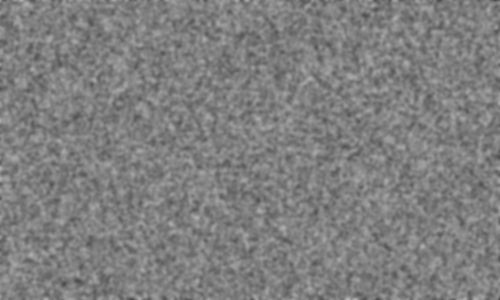
\includegraphics[width=.6\linewidth]{white-noise-blurred.jpg}
  \captionof{figure}{White noise blurred}
  \label{fig:test2}
\end{minipage}
\end{figure}

Una parte clave de este algoritmo es que puede ser repetido tantas veces como desea. Su único input es un punto 3D y siempre devuelve el mismo número aleatorio. Los puntos cercanos devuelven números próximos. Además, es simple y rápido.

La implementación usada en este trabajo está basada en la explicación de Andrew Kensler (ver \cite{perlinnoiseimplementation}) sobre cómo construir una función de ruido igual a la que describió Perlin.

El algoritmo original de Perlin usaba un interpolador de Hermite cúbico de la forma $s(t)=3t^2-2t^3$. Esta función es comunmente llamada \textit{smoothstep} por su forma de $s$ en el intervalo $[0,1]$. Además, es simétrica respecto del centro del cuadrado $[0,1]\times[0,1]$, lo que permite extenderla al intervalo $[-1,0]$, definiendo así $f(t)=1-s(|t|)=1-(3-2|t|)t^2$.

\inputtikz{hermite}

Esto es fácilmente extendible a dos y tres dimensiones si se aplica esta función a cada una de las variables y luego simplemente tomamos el producto. Por ejemplo, en 2D se tendrían puntos de la forma $(x,y)$, luego el ruido se formaría calculando $f(x)f(y)$. Si al 0 se le asigna el color negro, al 1 el blanco y al resto una escala de grises, se consigue un gradiente casi circular de blanco a negro.

\inputtikz{noise}

El problema ahora es que este ruido va a ser el mismo siempre. Por esa razón es necesario randomizarlo de alguna forma. Para ello, se toma un vector aleatorio partiendo del origen, y se multiplica con el punto $(x,y)$, considerado como vector. Es decir, sea $G$ un vector aleatorio partiendo del origen, el gradiente se calcularía como $f(x)f(y)(G\cdot(x,y))$.

Esta construcción tiene varias propiedades:
\begin{itemize}
\item Siempre hay una línea perpendicular al vector $G$ que pasa por el origen, donde el gradiante vale 0. Esto divide el cuadrado $[-1,1]\times[-1,1]$ en dos partes iguales: en una el gradiente es positiva y en otra negativo.
\item Rotar $G$ implica cambiar la dirección del gradiente.
\item Cambiar la longitud de $G$, modifica la intensidad del gradiente. Cuanto más largo $G$, más intenso será el gradiente, y al contrario. Por esta razón, se pueden coger simplemente vectores de longitud unidad.
\end{itemize}

Una vez se ha construido el elemento básico del ruido, simplemente hay que escoger un vector $G$ en cada uno de los puntos de la malla de enteros en el plano, es decir, los puntos $(n,m)$ donde $n,m\in\mathbb{N}$. Una vez escogidos, calcular el ruido sumando las contribuciones de cada vector (en 2D, serán cuatro, mientras que en 3D serán ocho).

\subsubsection{Implementación}

Como se ha visto en el apartado anterior, es necesario dividir $\mathbb{R}^3$ en cubos unitarios. Los vértices de esos cubos serán los puntos cuyas coordenadas sean enteras, es decir, los puntos $(i,j,k)\in\mathbb{R}^3$ donde $i,j,k\in\mathbb{N}$. A cada vértice se le asignará un vector unitario y aleatorio $G$. Para realizar esta elección es necesario crear un array conteniendo 256 vectores unitarios aleatorios (\textit{ranvec}) y tres arrays contenido 256 enteros (desde 0 hasta 255 sin repetir) permutados aleatoriamente  (\textit{perm\_x}, \textit{perm\_y} y \textit{perm\_z}).

\begin{lstlisting}[]
auto i = static_cast<int>(floor(p.x()));
auto j = static_cast<int>(floor(p.y()));
auto k = static_cast<int>(floor(p.z()));

vec3 c[2][2][2];

for (int di=0; di < 2; di++)
    for (int dj=0; dj < 2; dj++)
        for (int dk=0; dk < 2; dk++)
            c[di][dj][dk] = ranvec[
                perm_x[(i+di) & 255] ^
                perm_y[(j+dj) & 255] ^
                perm_z[(k+dk) & 255]
            ];
\end{lstlisting}

Hay varias cosas que deben ser comentadas en ese código:
\begin{itemize}
\item Tomar las partes enteras de las coordenadas del punto como índices favorece la aleatoriedad de la elección y minimiza los cambios bruscos de ruido en puntos próximos.
\item El uso de \textit{di}, \textit{dj} y \textit{dk} evita elegir dos veces el mismo vector para un mismo punto.
\item La operación $\& \;\; 255$ es necesario ya que las partes enteras de los puntos no tienen por qué estar entre 0 y 255.
\item El \textit{exclusive-or} ayuda a dispersar las elecciones de los vectores.
\end{itemize}

Básicamente lo que se ha construido con ese código es un hashing de puntos a vectores. Por último, falta calcular el valor de ruido asociado a cada vector y sumar cada contribución. En el apartado anterior no se ha hablado de interpolación trilineal, pero es necesario usarla para suavizar el resultado del ruido. En caso contrario, el resultado seguirá siendo un ruido de Perlin, pero visualmente tendrá una apariencia poligonal nada deseable.

\begin{lstlisting}[basicstyle=\footnotesize]
double perlin_interp(vec3 c[2][2][2], double u, double v, double w) {
    // maping to [-1,1]
    auto u = p.x() - floor(p.x());
    auto v = p.y() - floor(p.y());
    auto w = p.z() - floor(p.z());
    
    // hermite interpolation
    auto uu = u*u*(3-2*u);
    auto vv = v*v*(3-2*v);
    auto ww = w*w*(3-2*w);
    
    // trilinear interpolation + gradient
    auto accum = 0.0;
    for (int i=0; i < 2; i++)
        for (int j=0; j < 2; j++)
            for (int k=0; k < 2; k++) {
                vec3 weight_v(u-i, v-j, w-k);
                accum += (i*uu + (1-i)*(1-uu))*
                    (j*vv + (1-j)*(1-vv))*
                    (k*ww + (1-k)*(1-ww))*
                    dot(c[i][j][k], weight_v);
            }

    return accum;
}
\end{lstlisting}

La implementación de la interpolación trilineal fue propuesta por Paul Bourke en Julio de 1997 (ver \cite{paulbourke}).

\subsubsection{Modificaciones}

Dos modificaciones que pueden ser añadidas para crear, por ejemplo, texturas parecidas a la del mármol, son:

\begin{itemize}
\item Turbulencias: que no es mas que hacer una media ponderada de varios valores de ruido calculado sobre el mismo punto.
\item Ajustar frecuencias: hacer el color proporcional a algo que se asemeje a una función seno.
\end{itemize}

\section{Image Texture Mapping}

Desde el punto de intersección $P$, se calculan las coordenadas $(u,v)$ en la superficie. Después se usan esas coordenadas como índices en una textura sólida procedural (como el mármol creado en el apartado anterior) o como índices en los píxeles de una imagen.

Para lo último, una forma de directa es redondear $(u,v)$ a enteros y usar los píxeles $(i,j)$ correspondientes a la imagen. Esto presenta un problema ya que esa implementación depende de la resolución de la imagen, así que si se cambia la resolución también habría que cambiar esa parte del código. Para evitar este problema, se suele usar \textit{coordenadas de textura}, que son coordenadas en $[0,1]$  adaptables a cualquier resolución. Por ejempo, para el píxel $(i,j)$ de una imagen con resolución $N_x\times N_Y$, las coordenadas de textura serían:
\[
u=\frac{i}{N_x-1} \;\;\;\; v=\frac{j}{N_y-1}
\]
Algo importante a tener en cuenta, es la posición que representan las coordenadas $(u,v)$ en la imagen. $u$ va de izquierda a derecha, como era de esperar, pero $v$, va de abajo hacia arriba.

\inputtikz{texture-coordinates}

\nocite{*}
\bibliography{bibliography/bibliography}\addcontentsline{toc}{chapter}{Bibliografía}
\bibliographystyle{ieeetr}

\chapter*{}
\thispagestyle{empty}
\end{document}

\begin{thebibliography}{9}
\bibitem{first_book}
\url{https://raytracing.github.io/books/RayTracingInOneWeekend.html}
\bibitem{antialiasing}
\url{https://hardzone.es/reportajes/que-es/anti-aliasing-juegos/}
\bibitem{gamma_correction}
\url{https://en.wikipedia.org/wiki/Gamma_correction}
\bibitem{lambertian}
\url{https://en.wikipedia.org/wiki/Lambertian_reflectance}
\bibitem{beam}
\url{https://www.optics4kids.org/what-is-optics/reflection/the-reflection-of-light#:~:text=Polished%20metal%20surfaces%20reflect%20light,the%20metal%20surface%20is%20reflected.&text=The%20law%20of%20reflection%20requires,imaginary%20line%20(dashed%20in%20Fig.}
\bibitem{tikzmanual}
\url{https://www.bu.edu/math/files/2013/08/tikzpgfmanual.pdf}
\bibitem{snellslaw}
\url{https://en.wikipedia.org/wiki/Snell%27s_law}
\bibitem{schlickapproximation}
\url{https://en.wikipedia.org/wiki/Schlick%27s_approximation}
\bibitem{bvh}
\url{https://en.wikipedia.org/wiki/Bounding_volume_hierarchy}
\bibitem{aabb}
\url{https://en.wikipedia.org/wiki/Minimum_bounding_box}
\bibitem{perlinnoise}
\url{https://en.wikipedia.org/wiki/Perlin_noise}
\bibitem{perlinnoiseimplementation}
\url{http://eastfarthing.com/blog/2015-04-21-noise/}
\bibitem{trilinearinterpolation}
\url{https://en.wikipedia.org/wiki/Trilinear_interpolation}
\bibitem{machbands}
\url{https://en.wikipedia.org/wiki/Mach_bands}
\bibitem{hermitiansmoothing}
\url{https://en.wikipedia.org/wiki/Cubic_Hermite_spline}
\bibitem{paulbourke}
\url{http://paulbourke.net/miscellaneous/interpolation/}
\end{thebibliography}